%
% File naaclhlt2018.tex
%
%% Based on the style files for NAACL-HLT 2018, which were
%% Based on the style files for ACL-2015, with some improvements
%%  taken from the NAACL-2016 style
%% Based on the style files for ACL-2014, which were, in turn,
%% based on ACL-2013, ACL-2012, ACL-2011, ACL-2010, ACL-IJCNLP-2009,
%% EACL-2009, IJCNLP-2008...
%% Based on the style files for EACL 2006 by 
%%e.agirre@ehu.es or Sergi.Balari@uab.es
%% and that of ACL 08 by Joakim Nivre and Noah Smith

\documentclass[11pt,a4paper]{article}
\usepackage[hyperref]{naaclhlt2018}
\usepackage{times}
\usepackage{array}
\usepackage{rotating}
\usepackage{multirow}
\usepackage{longtable}
\usepackage{latexsym}
\usepackage{wasysym}
\usepackage[]{graphicx}


\usepackage{url}

\aclfinalcopy % Uncomment this line for all SemEval submissions

%\setlength\titlebox{5cm}
% You can expand the titlebox if you need extra space
% to show all the authors. Please do not make the titlebox
% smaller than 5cm (the original size); we will check this
% in the camera-ready version and ask you to change it back.

\newcommand\BibTeX{B{\sc ib}\TeX}

%Title format for system description papers by task participants
\title{THU-HCSI at SemEval-2019 Task 3: Hierarchical Ensemble Classification of Contextual Emotion in Conversation}
%Title format for task description papers by task organizers
%\title{SemEval-2018 Task [TaskNumber]:  [Task Name]}


\author{
  Xihao Liang, Ye Ma, Mingxing Xu \\
  Department of Computer Science \& Technology \\
  Tsinghua University, Beijing, China \\
  {\tt (liangxh16, ma-y17)@mails.tsinghua.edu.cn, xumx@tsinghua.edu.cn} \\
  %\And
  %  Ye Ma \\
  %   Affiliation / Address line 1 \\
  %  Affiliation / Address line 2 \\
  %  Affiliation / Address line 3 \\
  %  {\tt email@domain} \\
}

\date{}

\begin{document}
\maketitle
\begin{abstract}

In this paper, we describe our hierarchical ensemble system designed for the SemEval-2019 task3, {\em EmoContext}. In our framework, we trained three set of classifiers for four-emotion classification, {\em Happy-Sad-Angry} classification and {\em Others}-or-not classification respectively. Through three steps of voting, the predicted labels of these three sets of classifiers are combined to make the final prediction. Experiment results show that the ensemble approach manages to obtain better predictive performance in comparison with the base classifiers and our system has achieved the top 10 performance in the final evaluation of {\em EmoContext}.

\end{abstract}

\begin{table*}[t!]\small
\begin{center}
\begin{tabular}{c|c|c|c}
\hline
\bf Turn 1 & \bf Turn 2 & \bf Turn 3 & \bf label \\
\hline
I live in uttra khand & ohh nice! love that place! \wedge.\wedge & \smiley\smiley & happy \\
degreee & what degree \& where? & sryyy i really got to goo & others \\
\hline
\end{tabular}
\end{center}
\caption{\label{tab:sample} Example training samples in Train set.}
\end{table*}

\section{Introduction}

Sentiment analysis is a task to identify the emotion conveyed by written language. With the popularization of the Internet and instant message applications, text has become one of the most familiar media that people use to express their ideas and communicate with each other. Automatic emotion classification can help people and robots better understand the messages or comments written by other people and make proper responses, which makes this study field increasingly important.

Approaches to sentiment analysis can be classified into three categories: rule-based approaches, non-neural machine learning approaches and deep learning approaches. Significantly, neural networks have achieved state-of-art performance in many recent studies. \citet{Gupta2017A} used a LSTM-based model to identify the emotion in 3-turn conversations in Twitter but the turn information is not manipulated. For emotion detection on TV show transcripts, a sequence-based convolutional neural network which can make use of information in the previous lines was designed by \citet{Zahiri2017Emotion}. \citet{Hazarika2018} proposed a conversational memory network based on both CNN \cite{Lecun1998Convolutional} and gated recurrent unit \cite{DChungGCB14} to recognize emotion in dyadic dialogue videos, featuring its ability to manipulate the information of different speakers. Designing a proper structure of neural network to capture the information in different types of text data still remains a valuable topic.

In this paper, we describe our approach to SemEval-2019 task3, {\em EmoContext}, which aims to encourage more research of contextual emotion detection in textual conversation. Datasets of 3-turn conversations are provided and the participating systems are required to predict the contextual emotion of the last turn in the conversation: {\em Happy}, {\em Sad}, {\em Angry} or {\em Others}. The system performance is evaluated by the micro-averaged F1-score for {\em Happy}, {\em Sad} and {\em Angry} (hereinafter referred as {\em HSA}) on the given Test set. Our system is composed of three sets of CNN-based classifiers trained for four-emotion classification, {\em Happy-Sad-Angry} classification and {\em Others}-or-not classification respectively. Through three steps of voting, the predicted labels of the base classifiers are combined to make the final prediction. Our system has achieved F1-score of 0.7616 in the final evaluation on Test set, which is the top 10 performance out of 165 participating systems.

This paper is organized as follows. In Section~\ref{sec:data}, we describe the datasets provided by the task organizers. In Section~\ref{sec:system_desc}, our system and the strategies of training base classifiers are detailed. In Section~\ref{sec:experiments}, we present and discuss the evaluation results of our system and the base classifiers. Conclusion is given in Section~\ref{sec:conclusion}.

\begin{table}\small
\begin{center}
\begin{tabular}{c|c c c c}
\hline
\bf Dataset & \bf Others & \bf Happy & \bf Sad & \bf Angry \\
\hline
Train & 14948 & 4243 & 5463 & 5506 \\
Dev & 2338 & 142 & 125 & 150 \\
Test & 4677 & 284 & 250 & 298 \\
\hline
\end{tabular}
\end{center}
\caption{\label{tab:dataset} Class distribution in each dataset.}
\end{table}

\section{Data}
\label{sec:data}

Task organizers have released three datasets. Each sample in these datasets contains a 3-turn conversation(Table~\ref{tab:sample}), in which Turn 1 was written by User 1, Turn 2 is User 2's reply to Turn 1 and Turn 3 is User 1's reply to Turn 2. The emotion label of Turn 3 is manually annotated for each conversation, which is one of the four emotions: {\em Happy}, {\em Sad}, {\em Angry} and {\em Others}. Class distributions of these three datasets are shown in Table~\ref{tab:dataset}. As the Train set and Dev set are both allowed to be used for model training at the phase of final evaluation, these two datasets are combined (hereinafter referred as the training set) to develop our system.

\section{System Description}
\label{sec:system_desc}

\subsection{Preprocessing}

Through our observation of the 3-turn conversations in the datasets, we realize the writing style resembles that of the tweets and comments in Twitter, featuring emoticons, informal usage of language, spelling errors and so on. Hence, we utilized the tweet processor, {\em ekphrasis}\footnote{https://github.com/cbaziotis/ekphrasis} \cite{Baziotis2017SE1704}. The preprocessing steps include (1) Twitter-specific tokenization, (2) spell correction, (3) word normalization for numbers and dates, (4) annotation for all-capital words, elongated words and repeated punctuations, (5) conversion of emoticons to emotion labels.

\subsection{Word Embeddings}
\label{ssec:word_emb}

Word embedding is to capture semantic, syntactic and sentiment information of a word or token and represent it by a vector. We use the pretrained embedding model provided by \citet{Baziotis2018SE1803} \footnote{https://github.com/cbaziotis/ntua-slp-semeval2018} (hereinafter called NtuaW2V) in our system, which contains 300-dimensional vectors trained on Twitter messages that are also preprocessed by {\em ekphrasis}. In addition, we tried another pretrained model provided by \citet{Mikolov2013Distributed} \footnote{https://code.google.com/archive/p/word2vec/} (hereinafter called GoogleW2V), which containes 300-dimensional vectors trained on Google News dataset, in order to get an insight into the effect of different embedding models.

\subsection{Classifier}

Our system is composed of neural network classifiers with the same structure (Fig~\ref{fig:classifier}). The input to the classifier is a 3-turn conversation, treated as 3 sequences of tokens after the preprocessing step. An embedding layer is used to project the input to 3 sequences of vectors. This layer is initialized by the pretrained word embeddings mentioned in Section~\ref{ssec:word_emb}. For tokens that are not covered in the embedding model but occur in no less than two training samples, we randomly initialize the embedding vectors.

Each sequence of vectors is then fed into a CNN layer followed by max pooling respectively to get a vector as the representation of the corresponding turn. Three vectors are concatenated as the feature vector of the 3-turn conversation and it is then fed into a dense layer with rectified linear unit (ReLU) and another dense layer with softmax to get the probability distribution over all predicted classes.

\begin{table}\small
\begin{center}
\begin{tabular}{c|c}
\hline
\bf Name & \bf Value \\ 
\hline
\# of classifiers in each set  & 5 \\
$thr_{II}$ & 2  \\
$thr_{III}$ & 3 \\
\hline
std. of Gaussian noise & 0.1 \\
kernel size of CNN  & 5 \\
filter number of CNN & 128 \\
\# of cells of the first dense layer & 32 \\
dropout keep prob. & 0.5 \\
\em $l_2$ & 0.2 \\
initial learning rate & 0.005 \\
decay of learning rate & 0.9 \\
minibatch size & 100 \\
\hline
\end{tabular}
\end{center}
\caption{\label{tab:hyper_param} Configuration of our system.}
\end{table}

\subsection{Hierarchical Ensemble}
\label{ssec:ensemble}

In order the improve the predictive performance, we design three steps of voting to combine the predicted labels of base classifiers. Three sets of classifiers are trained. Set A is a set of four-emotion classifiers trained by the given dataset and the original labels. Set B is a set of triple classifiers trained only by the samples of {\em HSA}. Classifiers in Set C are binary classifiers, which are also trained by the given dataset but the labels for samples of {\em HSA} are changed to {\em Not Others}. 

First step is the majority voting in Set A to get the base predicted labels (hereinafter referred as Prediction I). At the second step, majority voting is applied to Set B and we change the predicted label to the new major vote if the sample is not predicted as {\em Others} in Prediction I and the voting count of the majorly voted class exceeds a given threshold $thr_{II}$, by which the prediction for {\em HSA} is refined. This set of predicted labels are hereinafter referred as Prediction II. At the third step, classifiers in Set C vote for each sample whether it belongs to {\em Others} or not. Then we change the predicted label to {\em Others} if more than $thr_{III}$ classifiers in Set C vote for {\em Others}. This set of predicted labels are used as the final prediction (hereinafter referred as Prediction III). We train several classifiers for voting at each step instead of using single classifier as the revision will be statistically more reliable.

\begin{figure}
\begin{center}
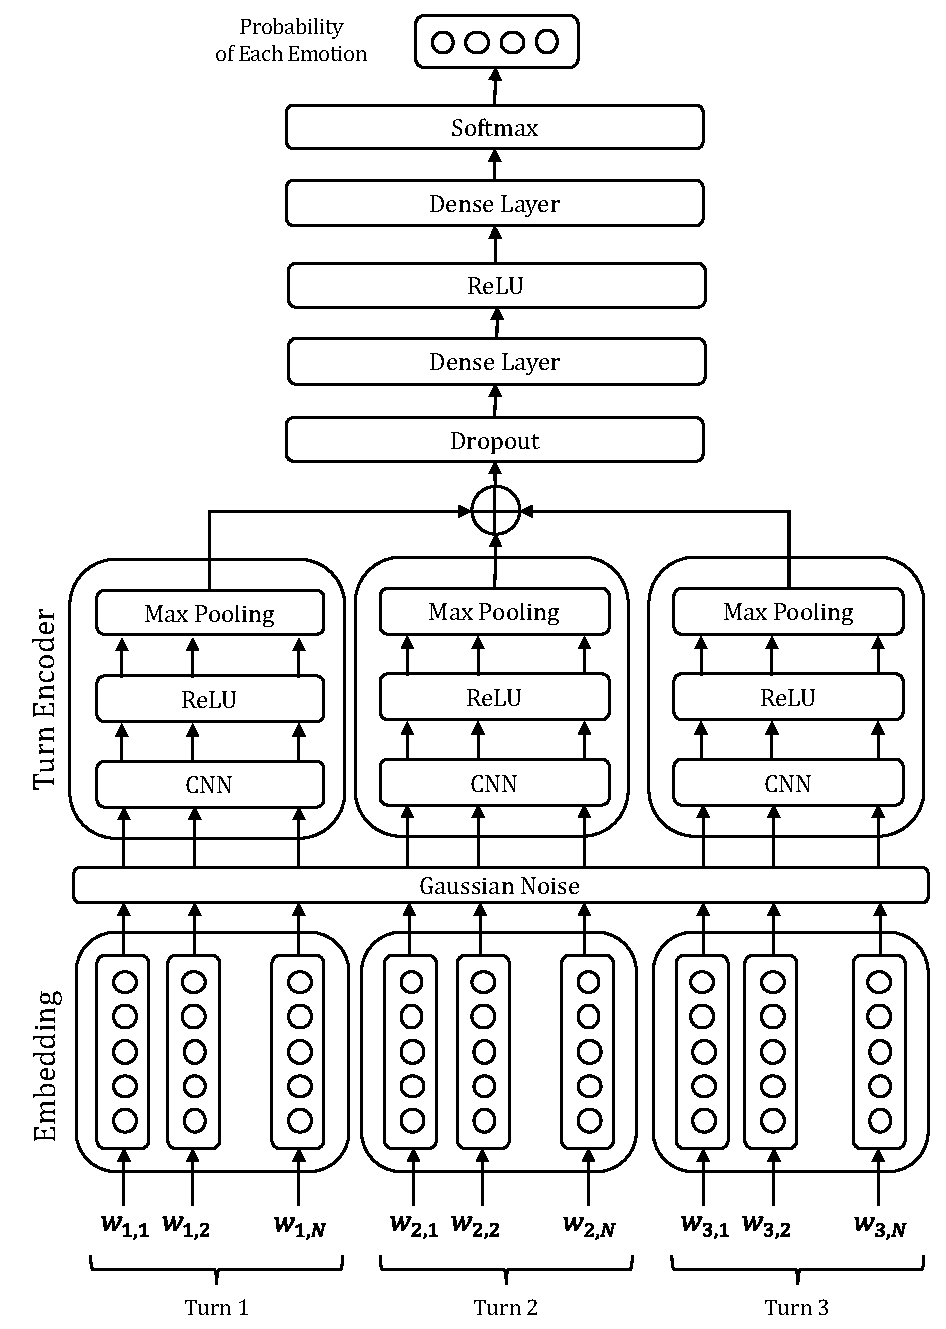
\includegraphics[width=0.45\textwidth]{framework_vertical.pdf}
\caption{\label{fig:classifier} The architecture of CNN-based classifiers in our system.}
\end{center}
\end{figure}

\subsection{Regularization}

In order to alleviate the problem of overfitting, following strategies are applied.

\begin{itemize}

\item Early stopping is used. For each classifier, we randomly select 90\% of the training set for training and the 10\% left for validation so that the information captured by each base classifier will diverse. Although the evaluation metric is micro-averaged F1 score for {\em Happy}, {\em Sad} and {\em Angry}, we choose the set of neural network weights that achieves the best micro-averaged precision on the validation set. As we notice that precision is significantly sensitive to the class distribution and the task organizers have emphasized the difference between the class distributions of the provides datasets in advance, we want the precision of the base classifiers to be as high as possible.

\item New samples of {\em Others} are automatically created. For each sample of the classs {\em Others} in the selected 90\% training set, we create a new {\em Others} sample by randomly remove one token in one of the turns to simulate the situation when the user misspell a word and that misspelled token is not known to our embedding models. As we observe that most of the {\em Others} samples in the training set still belong to {\em Others} even if one of the tokens is missing or misspelled. However, we do not generate samples for {\em Happy}, {\em Sad} and {\em Angry} automatically in case the discriminative token is removed and a missleading sample will be made.

\item Embedding layer is not fine-tuned as the relative positions of the embedding vectors of the tokens in the training set will be changed but those of the tokens in Test set but not in the training set are not adjusted, which may lead to wrong representation of the meaning of these tokens in the new embedding space.

\item Gaussian noise is added after the embedding layer, by which the model is more robust when dealing with tokens of similar meaning, as they are supposed to be projected to adjacent embedding vectors.

\item Dropout layer is added before the stacked dense layers (Fig~\ref{fig:classifier}).

\item L2 regularization is applied to the weights of the stacked dense layers.

\end{itemize}

\begin{table}\small
\begin{center}
\begin{tabular}{l|cccc}
\hline
\bf Classifier & \bf Acc & \bf Prec & \bf Rec & \bf F1 \\ 
\hline
Base  & \bf 0.9244 & 0.7247 & 0.7661 & \bf 0.7445 \\
\quad no extra Others & 0.9206 & 0.6974 & 0.7932 & 0.7420 \\
\hline
Early stopping & & & & \\
\quad F1-score & 0.9112 & 0.6521 & 0.8093 & 0.7222 \\
\quad Recall & 0.9020 & 0.6190 & \bf 0.8253 & 0.7073 \\
\hline
Emb \\
\quad GoogleW2V & 0.9226 & \bf 0.7421 & 0.7163 & 0.7286 \\
\hline
\end{tabular}
\end{center}
\caption{\label{tab:base_clfr} Performance of the base classifier and its variants on Test set.}
\end{table}

\section{Experiments and Discussion}
\label{sec:experiments}

\subsection{Implementation Details}

Tensorflow \cite{tensorflow} is used to develop our models. For network optimization, we choose Adam algorithm \cite{Kingma2014Adam}. Configuration of our system and the hyper-parameters of the base classifiers are shown in Table~\ref{tab:hyper_param}. 

\subsection{Results and Discussion}

Table~\ref{tab:base_clfr} shows the performance of our base classifier and its variants on the Test set. Note that {\bf Base} refers to the model trained as mentioned in Section~\ref{sec:system_desc} and {\bf Prec}, {\bf Rec} and {\bf F1} refers to the micro-averaged ones over {\em HSA}.

According to Table~\ref{tab:base_clfr}, adding automatically generated {\em Others} samples can improve the accuracy, precision and F1-score as more {\em Others} samples are correctly predicted but less {\em HAS} samples are recalled as the cost.

We also observe the performance difference when different metric is used as the indicator for choosing the network weights in early stopping, which is rarely discussed but the results show that the effect is significant. It is because of the remarkable difference between the class distributions of the training set and the Test set, which is emphasized by the task organizers.

On the other hand, NtuaW2V and GoogleW2V, the embedding models used to initialize the embedding layer, are compared. Results show that using NtuaW2V can achieve better F1-score while using GoogleW2V achieve the best precision but also the worst recall among the variants, which shows the importance of choosing suitable pretrained embedding models. The data on which the embedding model is trained and how the data are preprocessed should be the crucial keys to it.

% We have analyzed the base classifier's confusion matrix on Test set (Table~\ref{tab:conf_mat}) and two phenomenons are observed. First, the crucial problem that affect the performance of our classifiers is that many {\em Others} samples are falsely predicted, which severely lowers the precision as the proportion of {\em Others} are remarkably high in Test set. The second phenomenon is that our classifiers are relatively effective to classify samples among {\em Happy}, {\em Sad} and {\em Angry}.

Table~\ref{tab:boosting_mat} illustrates the performance of our system after each step of voting. Results show that the first two steps bring slight improvement on all four metrics and the final step improves F1-score by raising the precision at the cost of recall, which implies that, in comparison with Set A, classifiers in Set B are more effective to distinguish {\em HSA} samples and those in Set C are more precise to classify whether a sample belongs to {\em Others}. Although these classifier sets are all trained on the given dataset, Set B and Set C manage to work as a patch to Set A as they only focus on the simplified classification problems.

% \begin{table}[]\small
% \centering
% \begin{tabular}{c|c|cccc}
% \hline
% \multicolumn{2}{c|}{\multirow{2}} & \multicolumn{4}{c}{\bf Pred}    \\ \cline{3-6} 
% \multicolumn{2}{c|}{}      & \bf Others & \bf Happy & \bf Sad & \bf Angry  \\ \hline
% \multirow{4}{*}{\bf Gold}  & \bf Others     & 4423   & 74    & 70  & 110   \\
%                            & \bf Happy      & 77     & 200   & 5   & 2     \\
%                            & \bf Sad        & 29     & 1     & 207 & 13    \\
%                            & \bf Angry      & 40     & 1     & 2   & 255   \\ \hline
% \end{tabular}
% \caption{\label{tab:conf_mat} Sample of confusion matrix on Test set.}
% \end{table}

\begin{table}\small
\begin{center}
\begin{tabular}{c|cccc}
\hline
\bf Prediction & \bf Acc & \bf Prec & \bf Rec & \bf F1 \\ 
\hline
(Base) & 0.9244 & 0.7247 & 0.7661 & 0.7445 \\
I & 0.9278 & 0.7360 & 0.7740 & 0.7545 \\
II & 0.9281 & 0.7383 & \bf 0.7764 & 0.7569 \\
III & \bf 0.9305 & \bf 0.7553 & 0.7680 & \bf 0.7616 \\
\hline
\end{tabular}
\end{center}
\caption{\label{tab:boosting_mat} Performance of our system after each step of voting on Test set.}
\end{table}

\section{Conclusion and Future Work}
\label{sec:conclusion}

In this paper, we present our system used for SemEval2019 Task3, {\em EmoContext}. This system is composed of three sets of CNN-based neural network models trained for four-emotion classification, {\em Happy-Sad-Angry} classification and {\em Others}-or-not classification respectively. Three steps of voting are used to combine the predicted labels of the base classifiers and make the final prediction. Experiment results show that our training strategies are effective and the ensemble approach manages to improve the performance in comparison with the base classifiers. We highlight the importance of choosing pretrained embedding models and picking the right metric as indicator for choosing network weights in early stopping. In order to achieve better result based on our system, improving the performance of base classifier is crucial. The structure of neural networks and the features used as the input should be the fields that worth further exploration.

\bibliography{semeval2018}
\bibliographystyle{acl_natbib}

\end{document}